\documentclass[11pt]{beamer}
\usepackage[spanish]{babel}
\usepackage[utf8]{inputenc}
\usepackage{graphics}
\usepackage{listings}
\usepackage{array}
\usepackage{times}


\usetheme{CambridgeUS}
\usecolortheme{seagull}
\usefonttheme[onlylarge]{structurebold}

\author{Sebasti\'an Mancilla}
\institute[UTFSM]{Universidad T\écnica Federico Santa Mar\ía}
\date{\today}
\title{ClasTool Makefile}

%%%%%%%%%%%%%%%%%%%%%%%%%%%%%%%%%%%%%%%%%%%%%%%%%%%%%%%%%%%%%%%%%%%%%%%%%%%

\begin{document}

\begin{frame}
  \begin{center}
    \begin{tabular*}{\textwidth}%
      {>{\centering}m{0.1\textwidth}@{\extracolsep{\fill}}>{\centering}m{3in}%
      >{\centering}m{0.1\textwidth}}
      
\includegraphics[height=0.09\textwidth]{usm} &
      \textsc{\scriptsize{Universidad T\'ecnica Federico Santa Mar\'ia\\
      Departamento de F\'isica}\\
      \footnotesize{UTFSM ATLAS Grid Team}} &
      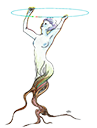
\includegraphics[height=0.1\textwidth]{root}
    \end{tabular*}

    \vspace{1.4cm}
    \large{\textbf{Nonrecursive Makefile for ClasTool}}

    \vspace{0.8cm}
    \normalsize{Sebasti\'an Mancilla Matta}\\
    \url{smancill@alumnos.inf.utfsm.cl}
  \end{center}
\end{frame}

%%%%%%%%%%%%%%%%%%%%%%%%%%%%%%%%%%%%%%%%%%%%%%%%%%%%%%%%%%%%%%%%%%%%%%%%%%%%%%

\begin{frame}
  \frametitle{Makefiles and make command}

  \textbf{make} is a utility intended to automate and optimize the
  construction of programs.

  \vspace{3mm}

  A descriptor file named \texttt{Makefile} describes the relationship among
  source files and provides commands for updating each file. 

  \pause
  \vspace{2mm}
  \begin{itemize}[<+->]
    \item \textbf{make} invokes \texttt{Makefile} to automatically rebuild a
      program whenever one of the source files is modified.\\[2mm]
    \item It only recompiles the files that were affected by changes, thus
      saving compiling time.\\[2mm]
    \item This helps reduce the likelihood of human errors when making entries
      from the command line.
  \end{itemize}
\end{frame}

%%%%%%%%%%%%%%%%%%%%%%%%%%%%%%%%%%%%%%%%%%%%%%%%%%%%%%%%%%%%%%%%%%%%%%%%%%%%%%

\lstset{%
     showstringspaces = false,
     basicstyle=\small\ttfamily,
   }

\begin{frame}[t,fragile]
  \frametitle{Makefiles and make command}
  \framesubtitle{Example}

  The executable \texttt{project1} is built from the following sources files:

  \vspace{5mm}
  \begin{lstlisting}[language=make]
         project
           |
           |_ main.c
           |_ data.h
           |_ data.c
           |_ io.h
           |_ io.c
  \end{lstlisting}

  \vspace{5mm}
  The source \texttt{main.c} includes \texttt{data.h} and
  \texttt{io.h}.

\end{frame}

%%%%%%%%%%%%%%%%%%%%%%%%%%%%%%%%%%%%%%%%%%%%%%%%%%%%%%%%%%%%%%%%%%%%%%%%%%%

\begin{frame}
  \frametitle{Makefiles and make command}
  \framesubtitle{Example}

  The dependencies between files are shown in the following tree:

  \begin{figure}[!htb]
    \centering
    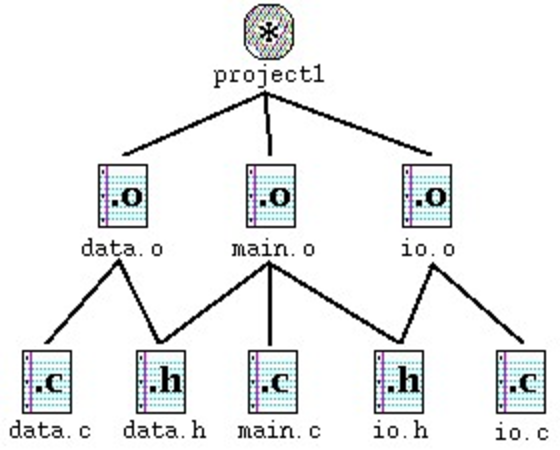
\includegraphics[width=0.6\textwidth]{dep_graph}
  \end{figure}

\end{frame}

%%%%%%%%%%%%%%%%%%%%%%%%%%%%%%%%%%%%%%%%%%%%%%%%%%%%%%%%%%%%%%%%%%%%%%%%%%%%%%

\begin{frame}[fragile]
  \frametitle{Makefiles and make command}
  \framesubtitle{Example}

  And this is a simple \texttt{Makefile} to build the executable:

  \vspace{5mm}
  \begin{lstlisting}[language=make, frame=single]
    project1: main.o data.o io.o
            gcc main.o data.o io.o -o project1

    main.o: data.h io.h main.c
            gcc -c main.c

    data.o: data.c data.h
            gcc -c data.c

    io.o: io.h io.c
            gcc -c io.c
  \end{lstlisting}
\end{frame}

%%%%%%%%%%%%%%%%%%%%%%%%%%%%%%%%%%%%%%%%%%%%%%%%%%%%%%%%%%%%%%%%%%%%%%%%%%%%%%

\begin{frame}[fragile]
  \frametitle{Makefiles and make command}
  \framesubtitle{Example}

  \small{
  \begin{itemize}
    \item \textbf{make} runs the rule for first target \texttt{project1} and
      figures its dependencies on \texttt{data.o}, \texttt{main.o} and
      \texttt{io.o}.
    \item \textbf{make} next checks if any of the three object files are
      listed as targets. If yes, it runs the rule for first prerequisite, that
      is, \texttt{main.o}, to find its dependencies.
    \item \textbf{make} checks whether the prerequisites of \texttt{main.o}
      have further dependencies. If not, as in the example, it checks if
      \texttt{main.o} is up to date. If not, it runs the command for
      \texttt{main.o} by compiling \texttt{main.c} to get the object file.
    \item \textbf{make} looks at the targets \texttt{data.o} and \texttt{io.o}
      and compiles these object files in a similar fashion.
    \item \textbf{make} returns to first target \texttt{project1}. Since it
      now has all up-to-date object files for the rule, it executes the
      command to build \texttt{project1}.
  \end{itemize}
  }

\end{frame}

%%%%%%%%%%%%%%%%%%%%%%%%%%%%%%%%%%%%%%%%%%%%%%%%%%%%%%%%%%%%%%%%%%%%%%%%%%%%%%
%%%%%%%%%%%%%%%%%%%%%%%%%%%%%%%%%%%%%%%%%%%%%%%%%%%%%%%%%%%%%%%%%%%%%%%%%%%%%%

\begin{frame}
  \frametitle{Recursive and nonrecursive Makefiles}

  \small{
  Traditionally the software development projects use a hierarchy of
  directories containing source files for the modules which make up the
  project.
  
  \vspace{2mm}
  \begin{itemize}[<+->]
    \item In the \textbf{recursive make} method each of the sub-directories
      contains a \texttt{Makefile} which describes the rules and instructions
      for the \textbf{make} program.

      The complete project build is done by arranging for the top-level
      \texttt{Makefile} to change directory into each of the sub-directories
      and recursively invoke \textbf{make}.\\[4mm]

    \item A \textbf{nonrecursive make} uses one single top-level
      \texttt{Makefile} to build the project and one \emph{make include file}
      for each sub-directory containing file lists and module-specific rules.
  \end{itemize}
  }
\end{frame}

%%%%%%%%%%%%%%%%%%%%%%%%%%%%%%%%%%%%%%%%%%%%%%%%%%%%%%%%%%%%%%%%%%%%%%%%%%%%%%
%%%%%%%%%%%%%%%%%%%%%%%%%%%%%%%%%%%%%%%%%%%%%%%%%%%%%%%%%%%%%%%%%%%%%%%%%%%%%%

\begin{frame}[label=issues]
  \frametitle{Recursive Makefile issues}
  Recursive makefiles are bad primarily because they partition the dependency
  tree into several trees.

  \begin{itemize}
    \item This prevents dependencies between make instances from being
      expressed correctly.\\[2mm]
    \item Also causes (parts of) the dependency tree to be recalculated
      multiple times, which is a performance issue in the end.
  \end{itemize}

  \vspace{5mm}
  This affects both phases of the operation of make:

  \begin{itemize}
    \item It causes make to construct an inaccurate dependency tree.\\[2mm]
    \item It forces make to traverse the tree in an inappropriate order.
  \end{itemize}

  \vspace{3mm}
  \hyperlink{tree-problem}{\beamergotobutton{Simple example of dependency problem}}
\end{frame}

%%%%%%%%%%%%%%%%%%%%%%%%%%%%%%%%%%%%%%%%%%%%%%%%%%%%%%%%%%%%%%%%%%%%%%%%%%%

\begin{frame}
  \frametitle{Recursive Makefile issues}
  Other problems include:

  \begin{itemize}
    \item Recursive makes which take \emph{forever} to work out that they need
      to do nothing.\\[2mm]
    \item Recursive makes which do too much, or too little.\\[2mm]
    \item Recursive makes which are overly sensitive to changes in the source
      code and require constant Makefile intervention to keep them
      working.\\[2mm]
    \item It is very hard to get the order of the recursion into the
      sub-directories correct.\\[2mm]
    \item It is often necessary to do more than one pass over the
      sub-directories to build the whole system.
  \end{itemize}
\end{frame}

%%%%%%%%%%%%%%%%%%%%%%%%%%%%%%%%%%%%%%%%%%%%%%%%%%%%%%%%%%%%%%%%%%%%%%%%%%%%%%
%%%%%%%%%%%%%%%%%%%%%%%%%%%%%%%%%%%%%%%%%%%%%%%%%%%%%%%%%%%%%%%%%%%%%%%%%%%%%%

\begin{frame}
  \frametitle{Using nonrecursive Makefiles}
  \begin{itemize}
    \item<1-> The use of a whole project make is not as difficult to put into
      practice as it may at first appear.\\[5mm]
    \item<2-> It solves the problems found in the recursive make approach.

      \begin{itemize}[<3->]
      \item It handles dependencies correctly. Treating the whole tree as a
        single entity is really the right way.\\[1mm]
      \item Specific targets can be built (say a particular program)
        correctly, since make always creates a full dependency graph.\\[1mm]
      \item It is faster.\\[5mm]
      \end{itemize}
    \item<4> It requires a paradigm shift for developers used to recursive
      make.
  \end{itemize}
\end{frame}

%%%%%%%%%%%%%%%%%%%%%%%%%%%%%%%%%%%%%%%%%%%%%%%%%%%%%%%%%%%%%%%%%%%%%%%%%%%%%%

\begin{frame}
  \frametitle{ROOT}
  \begin{itemize}
    \item The ROOT Makefile itself was structured as described in the paper
      \emph{Recursive Make Considered Harmful}.\\[5mm]
    \item The main philosophy is that it is better to have a single large
      Makefile describing the entire project than many small Makefiles, one
      for each sub-project, that are recursively called from the main
      Makefile. By cleverly using the include mechanism the single Makefile
      solution is as modular as the recursive approach without the problems of
      incomplete dependency graphs.\\[5mm]
    \item The single Makefile is fast.
      \begin{itemize}
        \item About 1 second to check if anything needs to be recompiled.
      \end{itemize}
  \end{itemize}
\end{frame}

%%%%%%%%%%%%%%%%%%%%%%%%%%%%%%%%%%%%%%%%%%%%%%%%%%%%%%%%%%%%%%%%%%%%%%%%%%%%%%
%%%%%%%%%%%%%%%%%%%%%%%%%%%%%%%%%%%%%%%%%%%%%%%%%%%%%%%%%%%%%%%%%%%%%%%%%%%%%%

\begin{frame}
  \frametitle{My approach for ClasTool}
  \begin{itemize}[<+->]
    \item I just took the old ClasTool Makefile and turned it into a
      nonrecursive Makefile.\\[4mm]
    \item My purpose was to eliminate the problems associated with using a
      recursive Makefile. 

      \begin{itemize}
        \item Because that is not the right way.\\[4mm]
      \end{itemize}

    \item All the dictionary, objects and dependency files are created inside
      of their source directory, so in the new approach this needs a series of
      specific rules for every directory.\\[4mm]
    \item The automatic dependency generation was inefficient, and with a
      couple of issues. 
  \end{itemize}
\end{frame}

%%%%%%%%%%%%%%%%%%%%%%%%%%%%%%%%%%%%%%%%%%%%%%%%%%%%%%%%%%%%%%%%%%%%%%%%%%%%%%

\begin{frame}
  \frametitle{Implementation}
  Three main files in the project root directory:

  \begin{itemize}
    \item \texttt{Makefile\_system:} it has all the system-dependent
      definitions (almost what \texttt{Makefile\_top} used to be).\\[2mm]
    \item \texttt{Makefile:} the project's nonrecursive Makefile.\\[2mm]
    \item \texttt{Makefile\_templates:} it has all the templates to build the
      specific rules for every directory, and the macros used by the
      \texttt{module.mk} files. 
  \end{itemize}

  \vspace{3mm}
  A \texttt{module.mk} file in each directory for building the libraries.

  \begin{itemize}
    \item All this files are included in the main Makefile.\\[2mm]
    \item All share the same structure.
  \end{itemize}
\end{frame}

%%%%%%%%%%%%%%%%%%%%%%%%%%%%%%%%%%%%%%%%%%%%%%%%%%%%%%%%%%%%%%%%%%%%%%%%%%%%%%

\lstset{%
     showstringspaces = false,
     basicstyle=\scriptsize\ttfamily,
   }

\begin{frame}[fragile]
  \frametitle{Implementation}
  Each \texttt{module.mk} file has the following lines:

  \begin{lstlisting}[language=make]
    local_class := $(wildcard $(module)/*.cc)
    local_files :=
    lib_name    := $(module)
    lib_deps    :=
    extra_libs  :=
    extra_flags :=


    $(eval $(call make-module,$(module),$(lib_name),$(lib_deps)))
    $(eval $(call make-libs,$(module),$(lib_name),$(lib_deps),    \
                            $(local_class),$(local_files),        \
                            $(extra_libs)))
    $(eval $(call make-objs,$(module),$(extra_flags)))
  \end{lstlisting}

  \pause
  For every directory the only thing that needs to be changed is the values of
  the variables. \texttt{\$(module)} is the name of the sub-directory.
\end{frame}

%%%%%%%%%%%%%%%%%%%%%%%%%%%%%%%%%%%%%%%%%%%%%%%%%%%%%%%%%%%%%%%%%%%%%%%%%%%%%%

\begin{frame}[fragile]
  \frametitle{Implementation}
  Each \texttt{module.mk} file has the following lines:

  \begin{lstlisting}[language=make]
    local_class := $(wildcard $(module)/*.cc)
    local_files :=
    lib_name    := $(module)
    lib_deps    := ClasBanks VirtualReader
    extra_libs  := -L$(ROOTLIBDIR) -lPhysics -lTree
    extra_flags := 


    $(eval $(call make-module,$(module),$(lib_name),$(lib_deps)))
    $(eval $(call make-libs,$(module),$(lib_name),$(lib_deps),    \
                            $(local_class),$(local_files),        \
                            $(extra_libs)))
    $(eval $(call make-objs,$(module),$(extra_flags)))
  \end{lstlisting}

  For every directory the only thing that needs to be changed is the values of
  the variables.
\end{frame}

%%%%%%%%%%%%%%%%%%%%%%%%%%%%%%%%%%%%%%%%%%%%%%%%%%%%%%%%%%%%%%%%%%%%%%%%%%%

\begin{frame}[label=eval]
  \frametitle{Implementation}
  \begin{itemize}
    \item The macros \texttt{make-module}, \texttt{make-libs} and
      \texttt{make-objs} are defined in \texttt{Makefile\_templates}.
      \hyperlink{make-libs}{\beamergotobutton{Example of a macro
      definition}}\\[4mm]
    \item By using the \texttt{eval} function, all the necessary rules are
      auto generated by make itself according to the above macros.\\[4mm]
    \item If some rules must be changed, this is done in one place:
      \texttt{Makefile\_templates}.\\[4mm]
    \item Auto-dependency generation is significantly improved using the
      advanced method invented by Tom
      Tromey\footnote{\url{http://make.paulandlesley.org/autodep.html}}.
  \end{itemize}
\end{frame}

%%%%%%%%%%%%%%%%%%%%%%%%%%%%%%%%%%%%%%%%%%%%%%%%%%%%%%%%%%%%%%%%%%%%%%%%%%%%%%

\begin{frame}
  \frametitle{Results}
  \begin{itemize}
    \item I hope all the work be useful.\\[5mm]
    \item As ClasTool, it is not finished, and it could be improved.\\[8mm]
    \item<2> But right now it works very good.
  \end{itemize}
\end{frame}

%%%%%%%%%%%%%%%%%%%%%%%%%%%%%%%%%%%%%%%%%%%%%%%%%%%%%%%%%%%%%%%%%%%%%%%%%%%%%%
%%%%%%%%%%%%%%%%%%%%%%%%%%%%%%%%%%%%%%%%%%%%%%%%%%%%%%%%%%%%%%%%%%%%%%%%%%%%%%

\begin{frame}[t]
  \frametitle{References}

  \begin{thebibliography}{99}
    \bibitem {RMH} \emph{Recursive Make Considered Harmful}, Peter Miller,
      1997\\
      \url{http://miller.emu.id.au/pmiller/books/rmch/}\\[7mm]
    \bibitem {MPM} \emph{Managing Projects with GNU make}, 3rd Edition, Robert
      Mecklenburg, 2004\\
      \url{http://www.makelinux.net/make3/main.html}\\[7mm]
    \bibitem {GIT} My Git repository (here you can find the sources)\\
      \url{http://github.com/smancill/ClasTool_Makefile}
  \end{thebibliography}
\end{frame}


%%%%%%%%%%%%%%%%%%%%%%%%%%%%%%%%%%%%%%%%%%%%%%%%%%%%%%%%%%%%%%%%%%%%%%%%%%%%%%
%%%%%%%%%%%%%%%%%%%%%%%%%%%%%%%%%%%%%%%%%%%%%%%%%%%%%%%%%%%%%%%%%%%%%%%%%%%%%%

\begin{frame}[label=tree-problem]
  \frametitle{Recursive Makefile dependencies problem}

  Suppose \textbf{make} is called first for \texttt{ModuleA} and then for
  \texttt{ModuleB}.

  \begin{figure}[!htb]
    \centering
    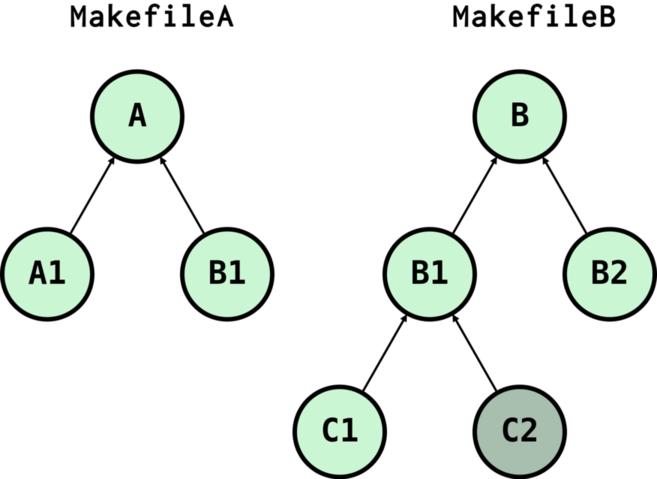
\includegraphics[width=0.5\textwidth]{dep_problem}
  \end{figure}


  What happens if we modified file \texttt{C2} and we call \textbf{make}
  command?

  \vspace{3mm}
  \hyperlink{issues}{\beamerreturnbutton{Back}}
\end{frame}

%%%%%%%%%%%%%%%%%%%%%%%%%%%%%%%%%%%%%%%%%%%%%%%%%%%%%%%%%%%%%%%%%%%%%%%%%%%%%%

\begin{frame}[fragile,label=make-libs]
  \frametitle{Example: make-libs macro}

  \begin{lstlisting}[language=make]
  define make-libs
  SOURCES_DEPS += $(call dep-list,$(1),$(4) $(5))
  SOURCES_DICTS += $(call dict-list,$(1),$(4))

  $(SLIBDIR)/lib$(2).$(DllSuf): $(call obj-list,$(1),$(4) $(5))  \
                                $(call dict-obj-list,$(1),$(4))
          @echo CREATING SHARED LIBRARY $$@
  ifeq (,$(7))
          $(LD) $(SOFLAGS) $(LDFLAGS) -o $$@       \
          $$^ $(6) $(if $3,-L$(SLIBDIR) $(addprefix -l,$3))
  else
          $(7) $(SOFLAGS) $(LDFLAGS) -o $$@        \
          $$^ $(6) $(if $3,-L$(SLIBDIR) $(addprefix -l,$3))
  endif
          $(POST_LINK_COMMAND)

  $(LIBDIR)/lib$(2).a: $(call obj-list,$(1),$(4) $(5))           \
                       $(call dict-obj-list,$(1),$(4))
          @echo CREATING LIBRARY $$@
          ar r $$@ $$^
  endef
  \end{lstlisting}
  \hyperlink{eval}{\beamerreturnbutton{Back}}
\end{frame}

\end{document}
